\section{Fonctionnalités} 


    
    \frame{\sectionpage}
    
   
    \begin{frame}{Géolocalisation}
        \centering
        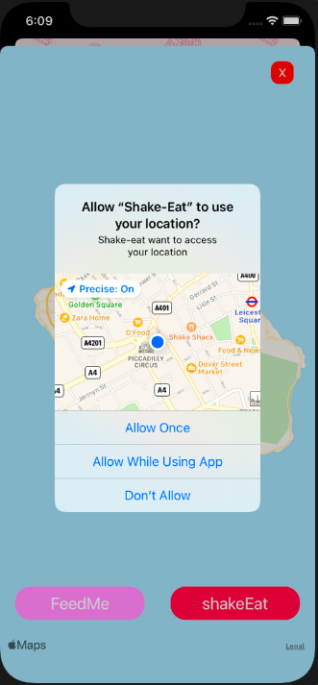
\includegraphics[height = 0.8 \textheight]{images/geoloc.png}
        
    \end{frame}
    
     \begin{frame}{La carte : Affichage des restaurants du coin}
        \centering
        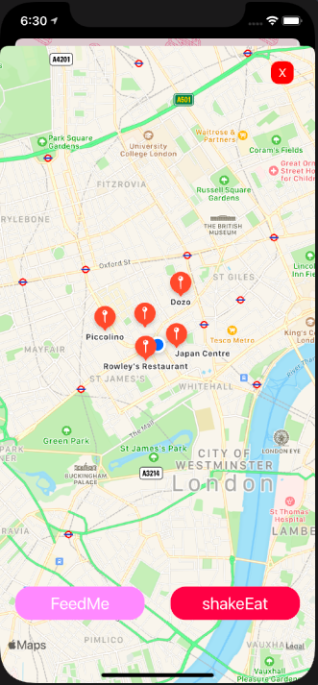
\includegraphics[width = 0.25\textwidth]{images/carte-tous-restos.png}
    \end{frame}
    
    \begin{frame}{Code Intéressant : choix aléatoire d'un point}
        \centering
            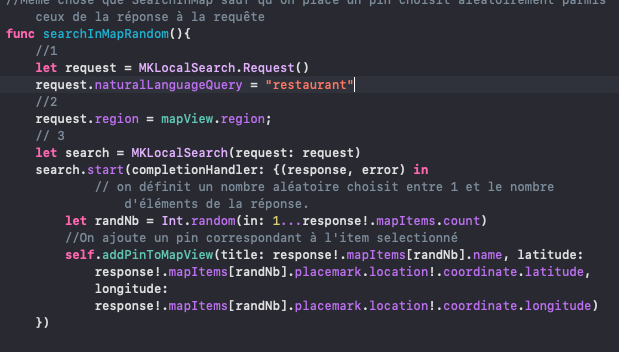
\includegraphics[height = 0.6 \textheight]{images/code-aleatoire.png}
    \end{frame}
    
    
    \begin{frame}{Pop-Up}
        La Pop-Up demande à l'utilisateur de secouer son téléphone
        \centering
        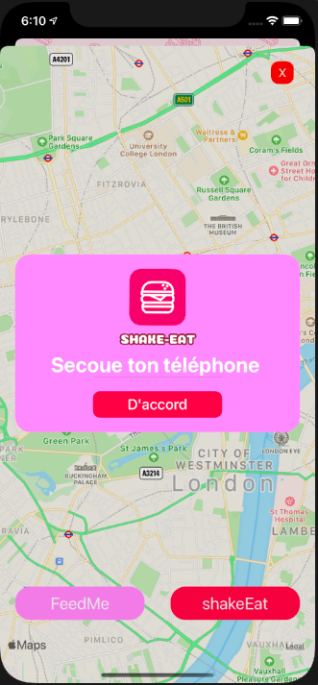
\includegraphics[width = 0.25\textwidth]{images/carte-post-shake.png}
    \end{frame}
    
    \begin{frame}{Post shake}
        Un restaurant est choisi au hasard parmi ceux dans le périmètre défini 
        \centering
        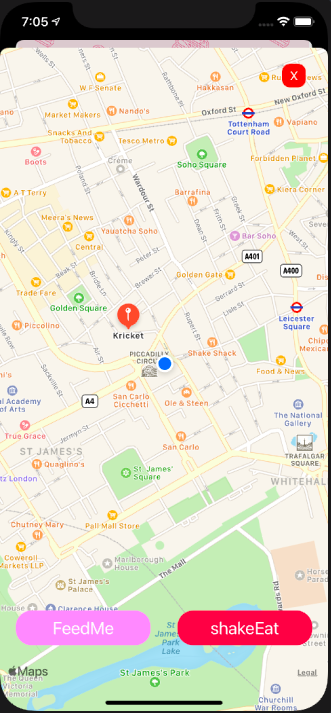
\includegraphics[width = 0.25\textwidth]{images/Shaked.png}
    \end{frame}
    
    
    
    
    
    